\documentclass[12pt,a4paper]{article}

% ---------- Packages ----------
\usepackage[UTF8]{ctex} % Chinese support for XeLaTeX
\usepackage{geometry}
\usepackage{setspace}
\usepackage{hyperref}
\usepackage{pdfpages}   % For inserting PDFs

% ---------- Page Setup ----------
\geometry{margin=0.8in}
\setstretch{1.25}


% ---------- Title ----------
\title{
    \vspace{-2cm} % Reduce space above the title
    {\Huge \textbf{Proof Documents Collection}}\\[0.3cm]
    {\Large Southern University of Science and Technology (SUSTech)}
    \vspace{-0.5cm} % Reduce space below the title
}
\author{By Lucky Chen}
\date{\today}

% ---------- Document ----------
\begin{document}

\maketitle
\thispagestyle{empty}

\noindent \textbf{Instructions / 使用须知:}

\begin{itemize}
    \item First, fill in your information, then send the PDF to the official email or the corresponding secretary for confirmation. 请先填写好信息,然后通过邮件发送 PDF 给各中心的官方邮箱或相关秘书确认。
    \item If you do not receive a timely reply, print this document and visit the office in person to get detailed instructions and the official stamp (\textbf{盖章}). 如果未及时收到回复,请直接打印文件并线下到办公室咨询并盖章。
    \item Note: Some centers (e.g., Sports Center) may prefer bilingual formatting: one line in Chinese, one line in English.
    \item For full Chinese support, please compile with \textbf{XeLaTeX}. 如需中文支持,请使用 XeLaTeX 编译;或直接使用提供的 Word 模板。
    \item You are encouraged to register for \textbf{语言指导服务} at the SUSTech Center for Language Education (CLE); they are very helpful with all kinds of application materials!
\end{itemize}

\noindent \textbf{Overleaf Online View:} \\
You can preview and download this document directly online via Overleaf: \\
\href{https://www.overleaf.com/read/kxgcyytxrkqf#8b3bc4}{\texttt{https://www.overleaf.com/read/kxgcyytxrkqf\#8b3bc4}}

\vspace{0.5cm}
\noindent \textbf{Disclaimer / 免责声明:} \\
This document is provided as a personal reference only. Please verify the final content and usage requirements with each relevant office. \\
本文件仅供个人申请参考,请以各部门实际要求为准,若因使用本文件产生任何后果,均与本人无关,本人不承担任何责任。

\vspace{0.5cm}
\noindent \textbf{Good Luck! / 祝一切顺利!} \\
May your applications go smoothly and your efforts be rewarded with success.\\祝大家申请顺利,前程似锦!

\vspace{0.5cm}

\noindent \textbf{If you find this kit helpful, please consider giving it a star on GitHub: \\
\href{https://github.com/LuckyChen3141/Sustech-Proof-Kit}{\texttt{https://github.com/LuckyChen3141/Sustech-Proof-Kit}}}

\newpage

% ---------- Content ----------
\section{Scholarship Proof}
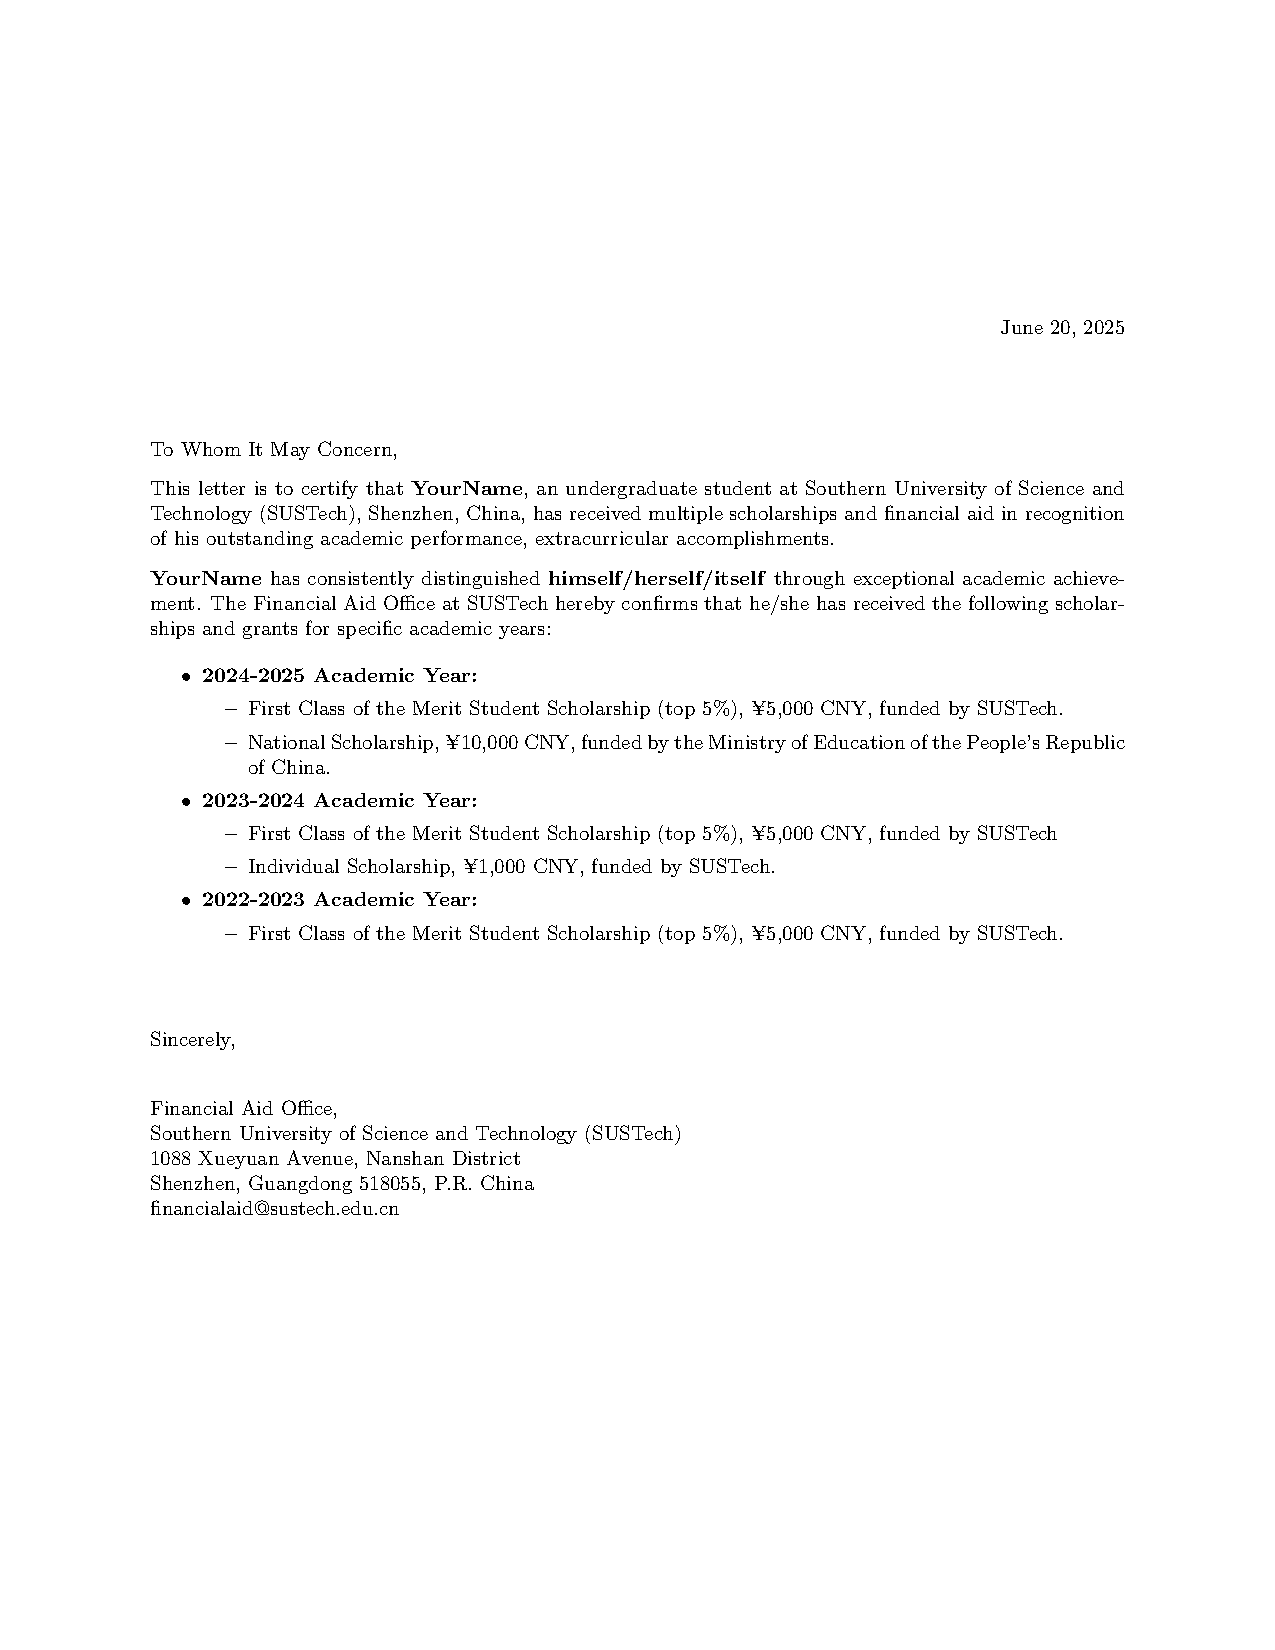
\includepdf[pages=-]{proofs/ScholarshipProof_FinancialAidOffice.pdf}

\section{Sports Awards Proof}
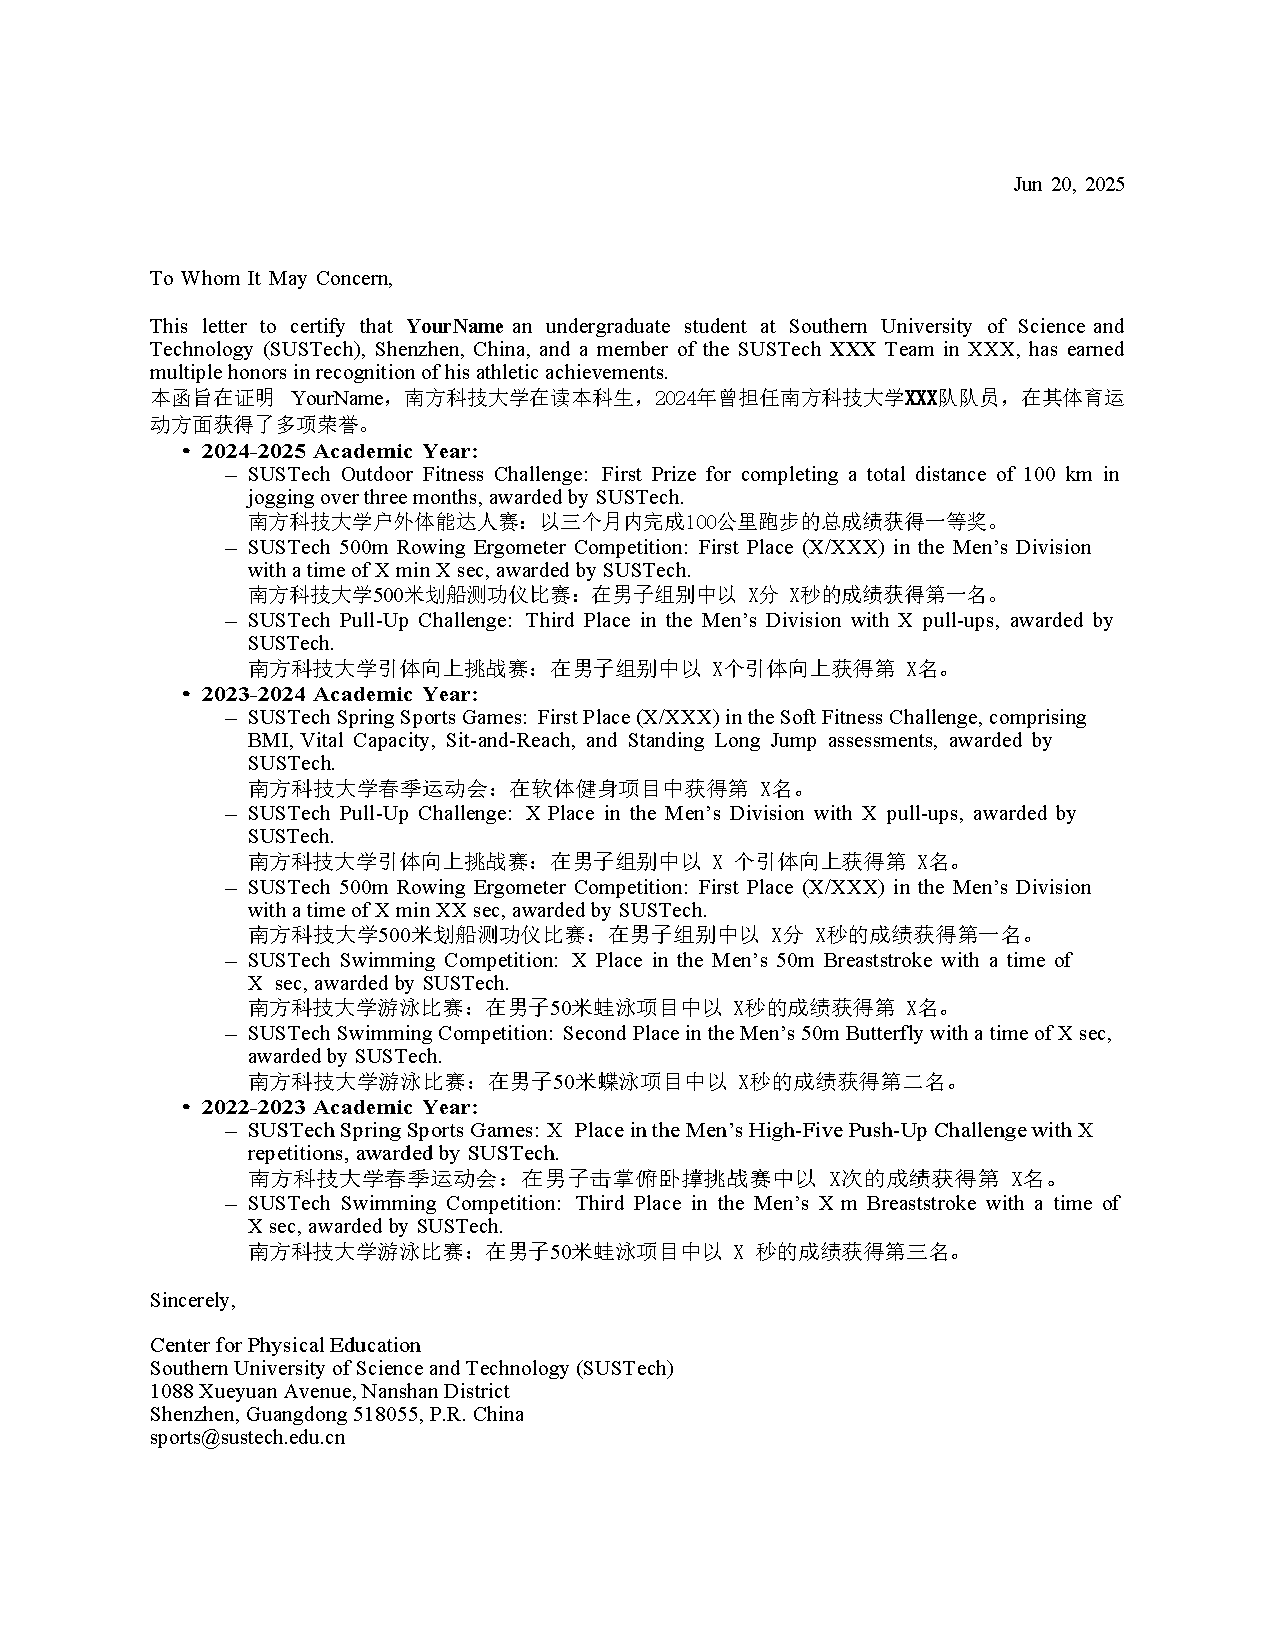
\includepdf[pages=-]{proofs/SportsAwardsProof_SportsCenter.pdf}

\section{SUSTech Admission Scholarship Proof}
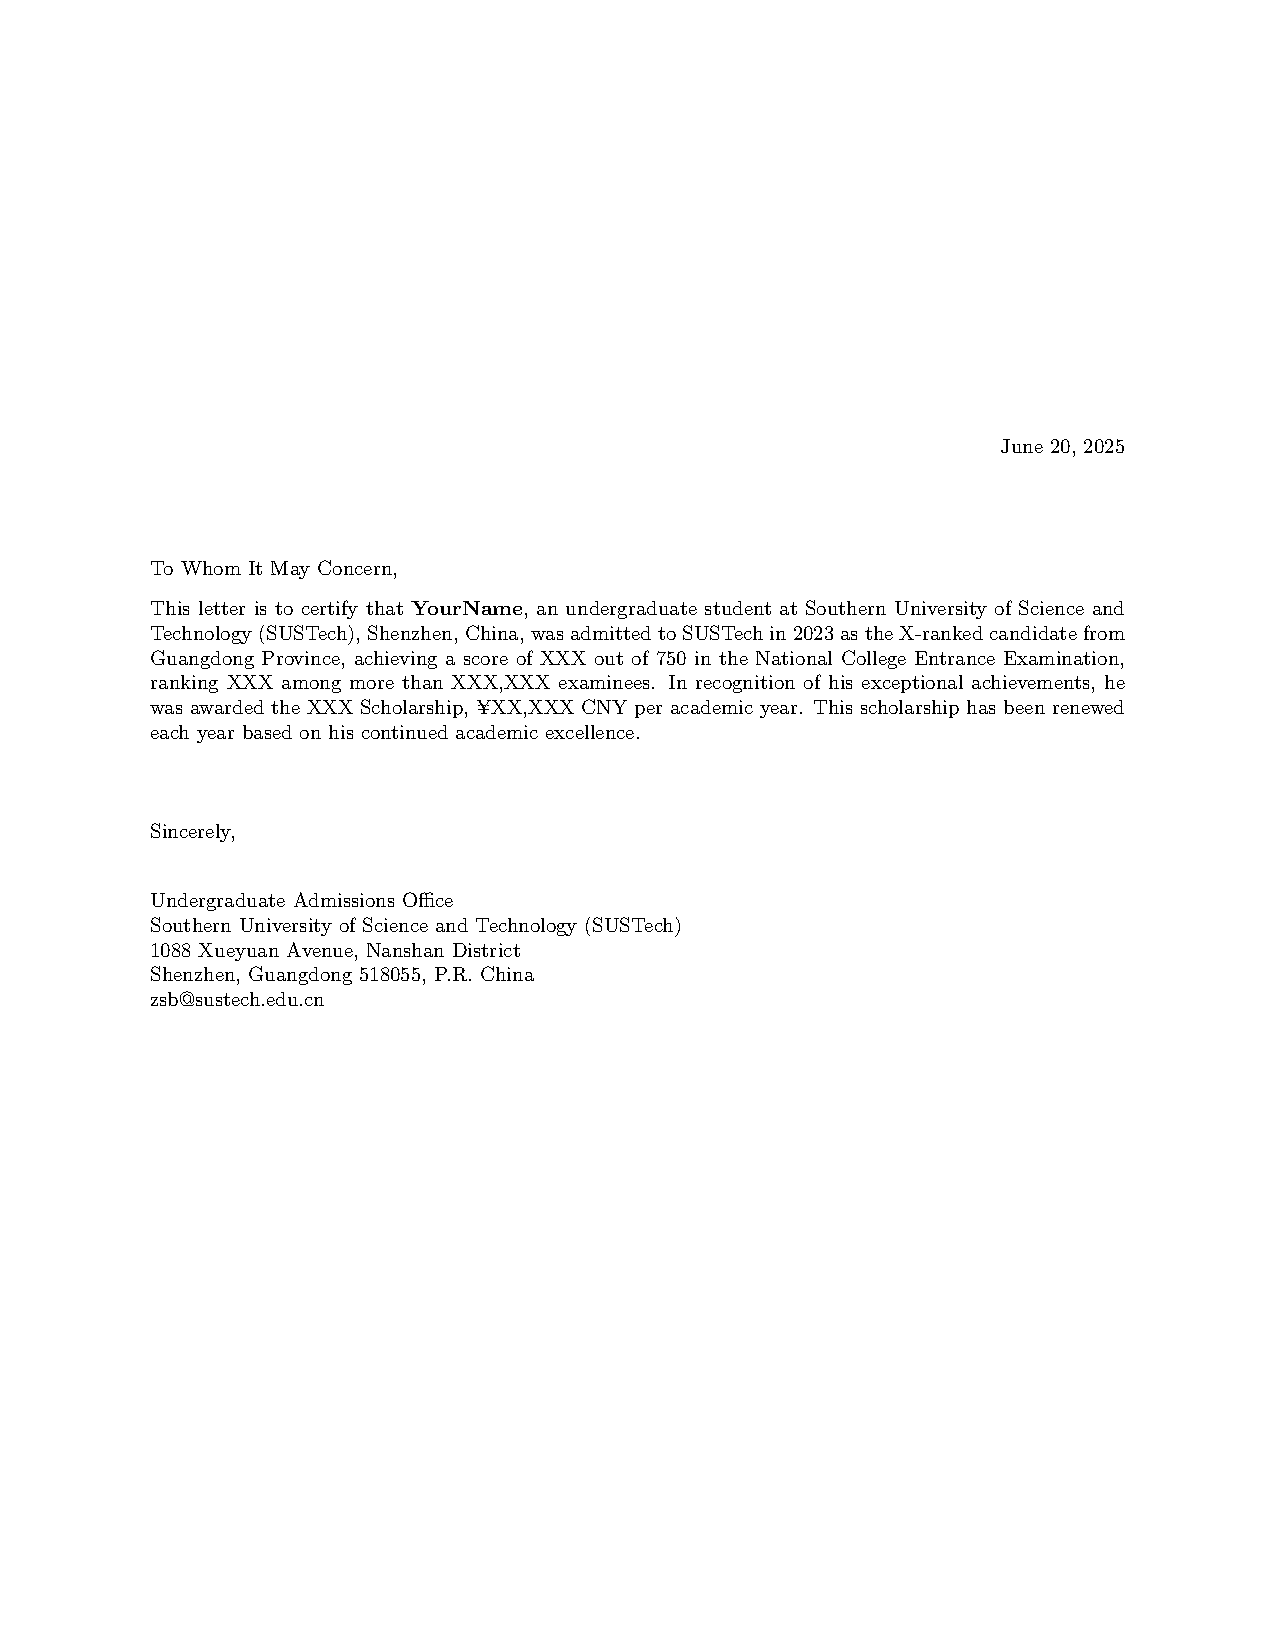
\includepdf[pages=-]{proofs/SUSTechAdmissionScholarshipProof_AdmissionOffice.pdf}

\section{SUSTech Volunteer Service Proof}
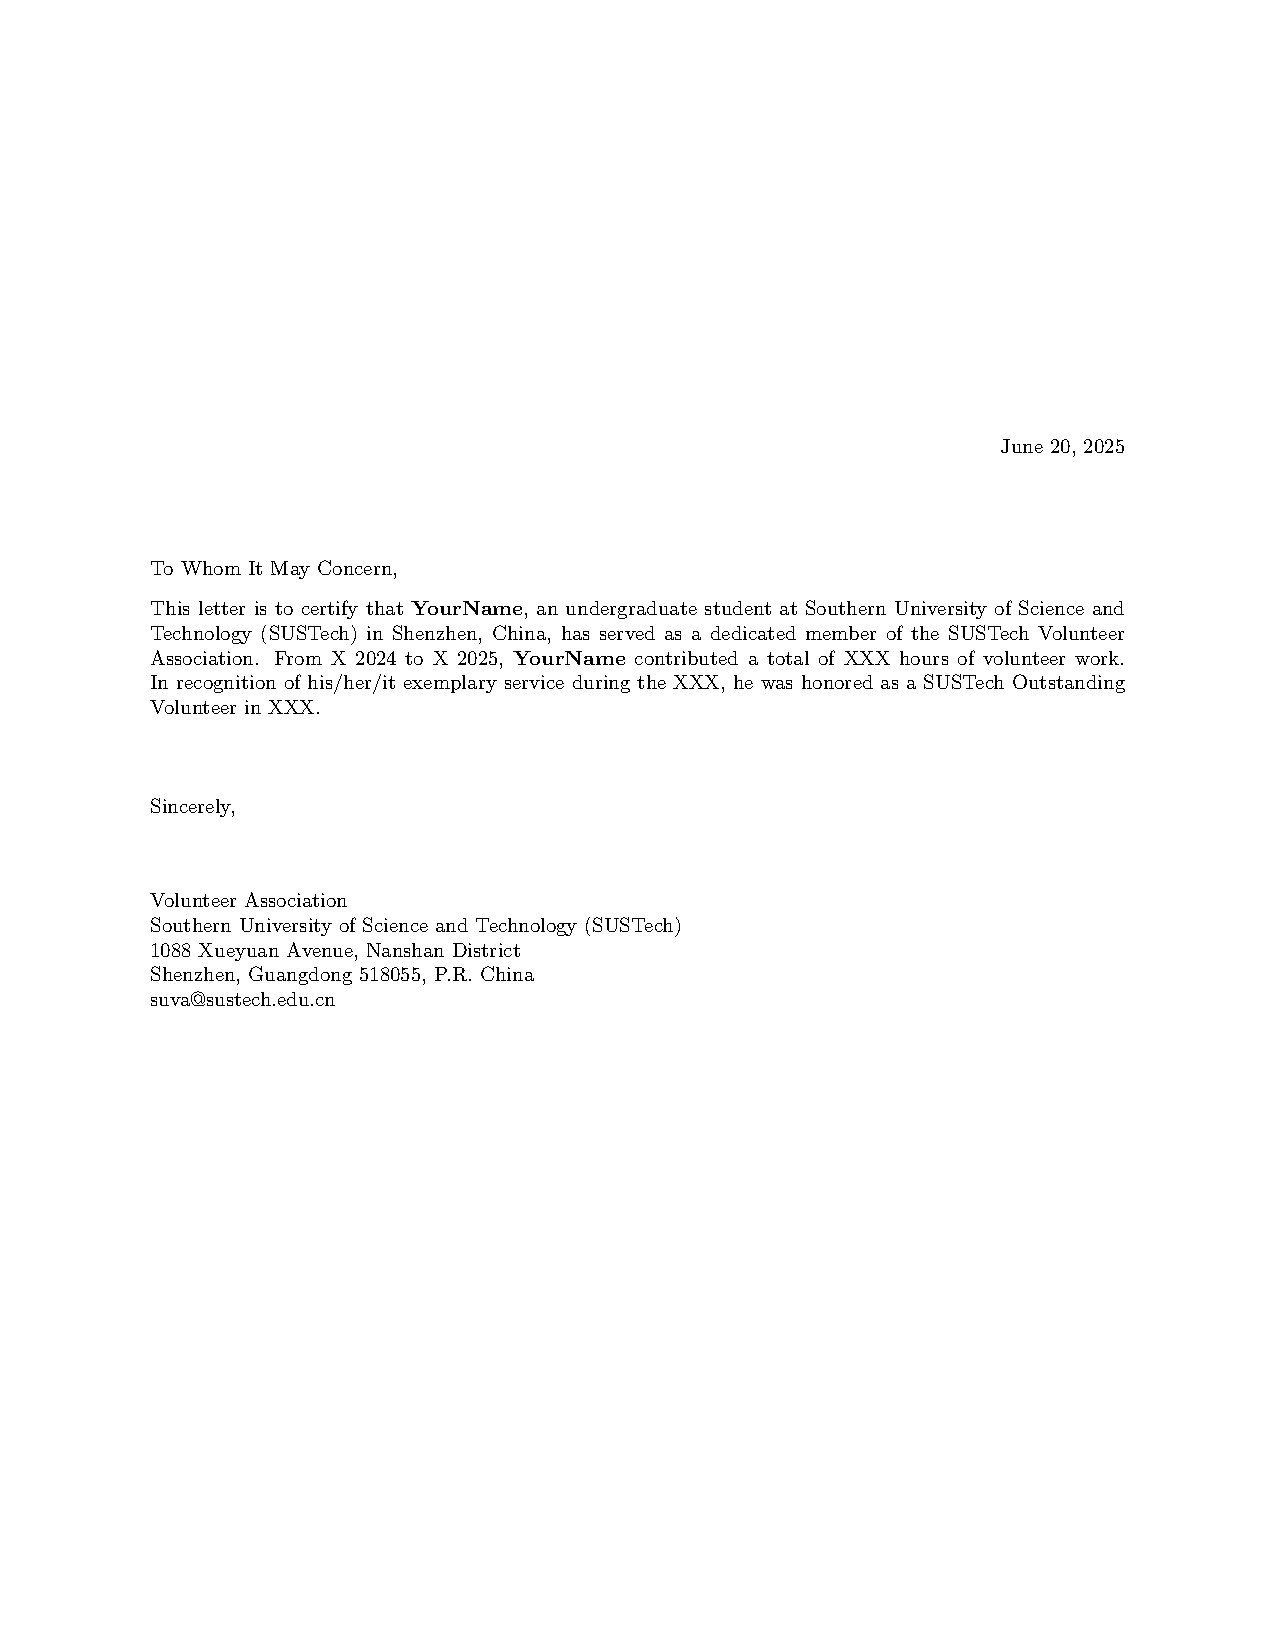
\includepdf[pages=-]{proofs/SUSTechVolunteerProof-SUSTechVolunteerAssociation.pdf}

% ---------- End ----------
\end{document}